\usetikzlibrary{calc,arrows.meta,patterns,angles,quotes}
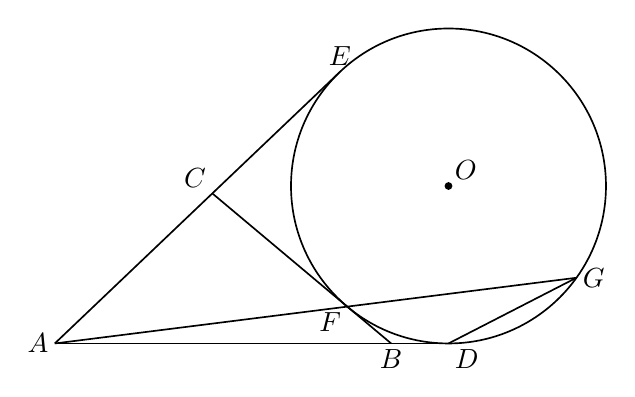
\begin{tikzpicture}[x=1cm,y=1cm,line width=.6pt,font=\normalsize,>=Stealth]
\coordinate (O) at (0.0000000000,2.0000000000);
\coordinate (A) at (-5.0000000000,0.0000000000);
\coordinate (D) at (0.0000000000,0.0000000000);
\coordinate (E) at (-1.3793103448,3.4482758621);
\coordinate (F) at (-1.2855752194,0.4679111138);
\coordinate (B) at (-0.7279404685,0.0000000000);
\coordinate (C) at (-2.9990385550,1.9056775667);
\coordinate (G) at (1.6253805169,0.8346081452);
\draw (O) circle[radius=2.0000000000cm];
\draw (A)--(E);
\draw (A)--(D);
\draw (B)--(C);
\draw (A)--(G);
\draw (G)--(D);
\fill (O) circle[radius=1.4pt];
\node[left=2pt,inner sep=0pt] at (A) {$A$};
\node[below right=2pt,inner sep=0pt] at (D) {$D$};
\node[above=2pt,inner sep=0pt] at (E) {$E$};
\node[below=2pt,inner sep=0pt] at (B) {$B$};
\node[above left=2pt,inner sep=0pt] at (C) {$C$};
\node[below left=2pt,inner sep=0pt] at (F) {$F$};
\node[right=2pt,inner sep=0pt] at (G) {$G$};
\node[above right=2pt,inner sep=0pt] at (O) {$O$};
\end{tikzpicture}
